\documentclass{ctexart} 
\usepackage{graphicx}
\usepackage{caption}
% 生成大图的标题包
\usepackage{subfigure}
% 生成子图的包
\begin{document} 
\begin{figure}[htbp]
    \centering  %居中
    \subfigure[name of the subfigure]{   %第一张子图
    \begin{minipage}{0.4\textwidth}%大小总和超过textwidth则自动换行
    \centering    %子图居中
    
\includegraphics[width=\textwidth]{3.png}  %设置图片的输出大小倍数,这里是0.5倍大小输出
    \end{minipage}
    }
    \subfigure[name of the subfigure]{ %第二张子图
    \begin{minipage}{0.4\textwidth}
    \centering    %子图居中
    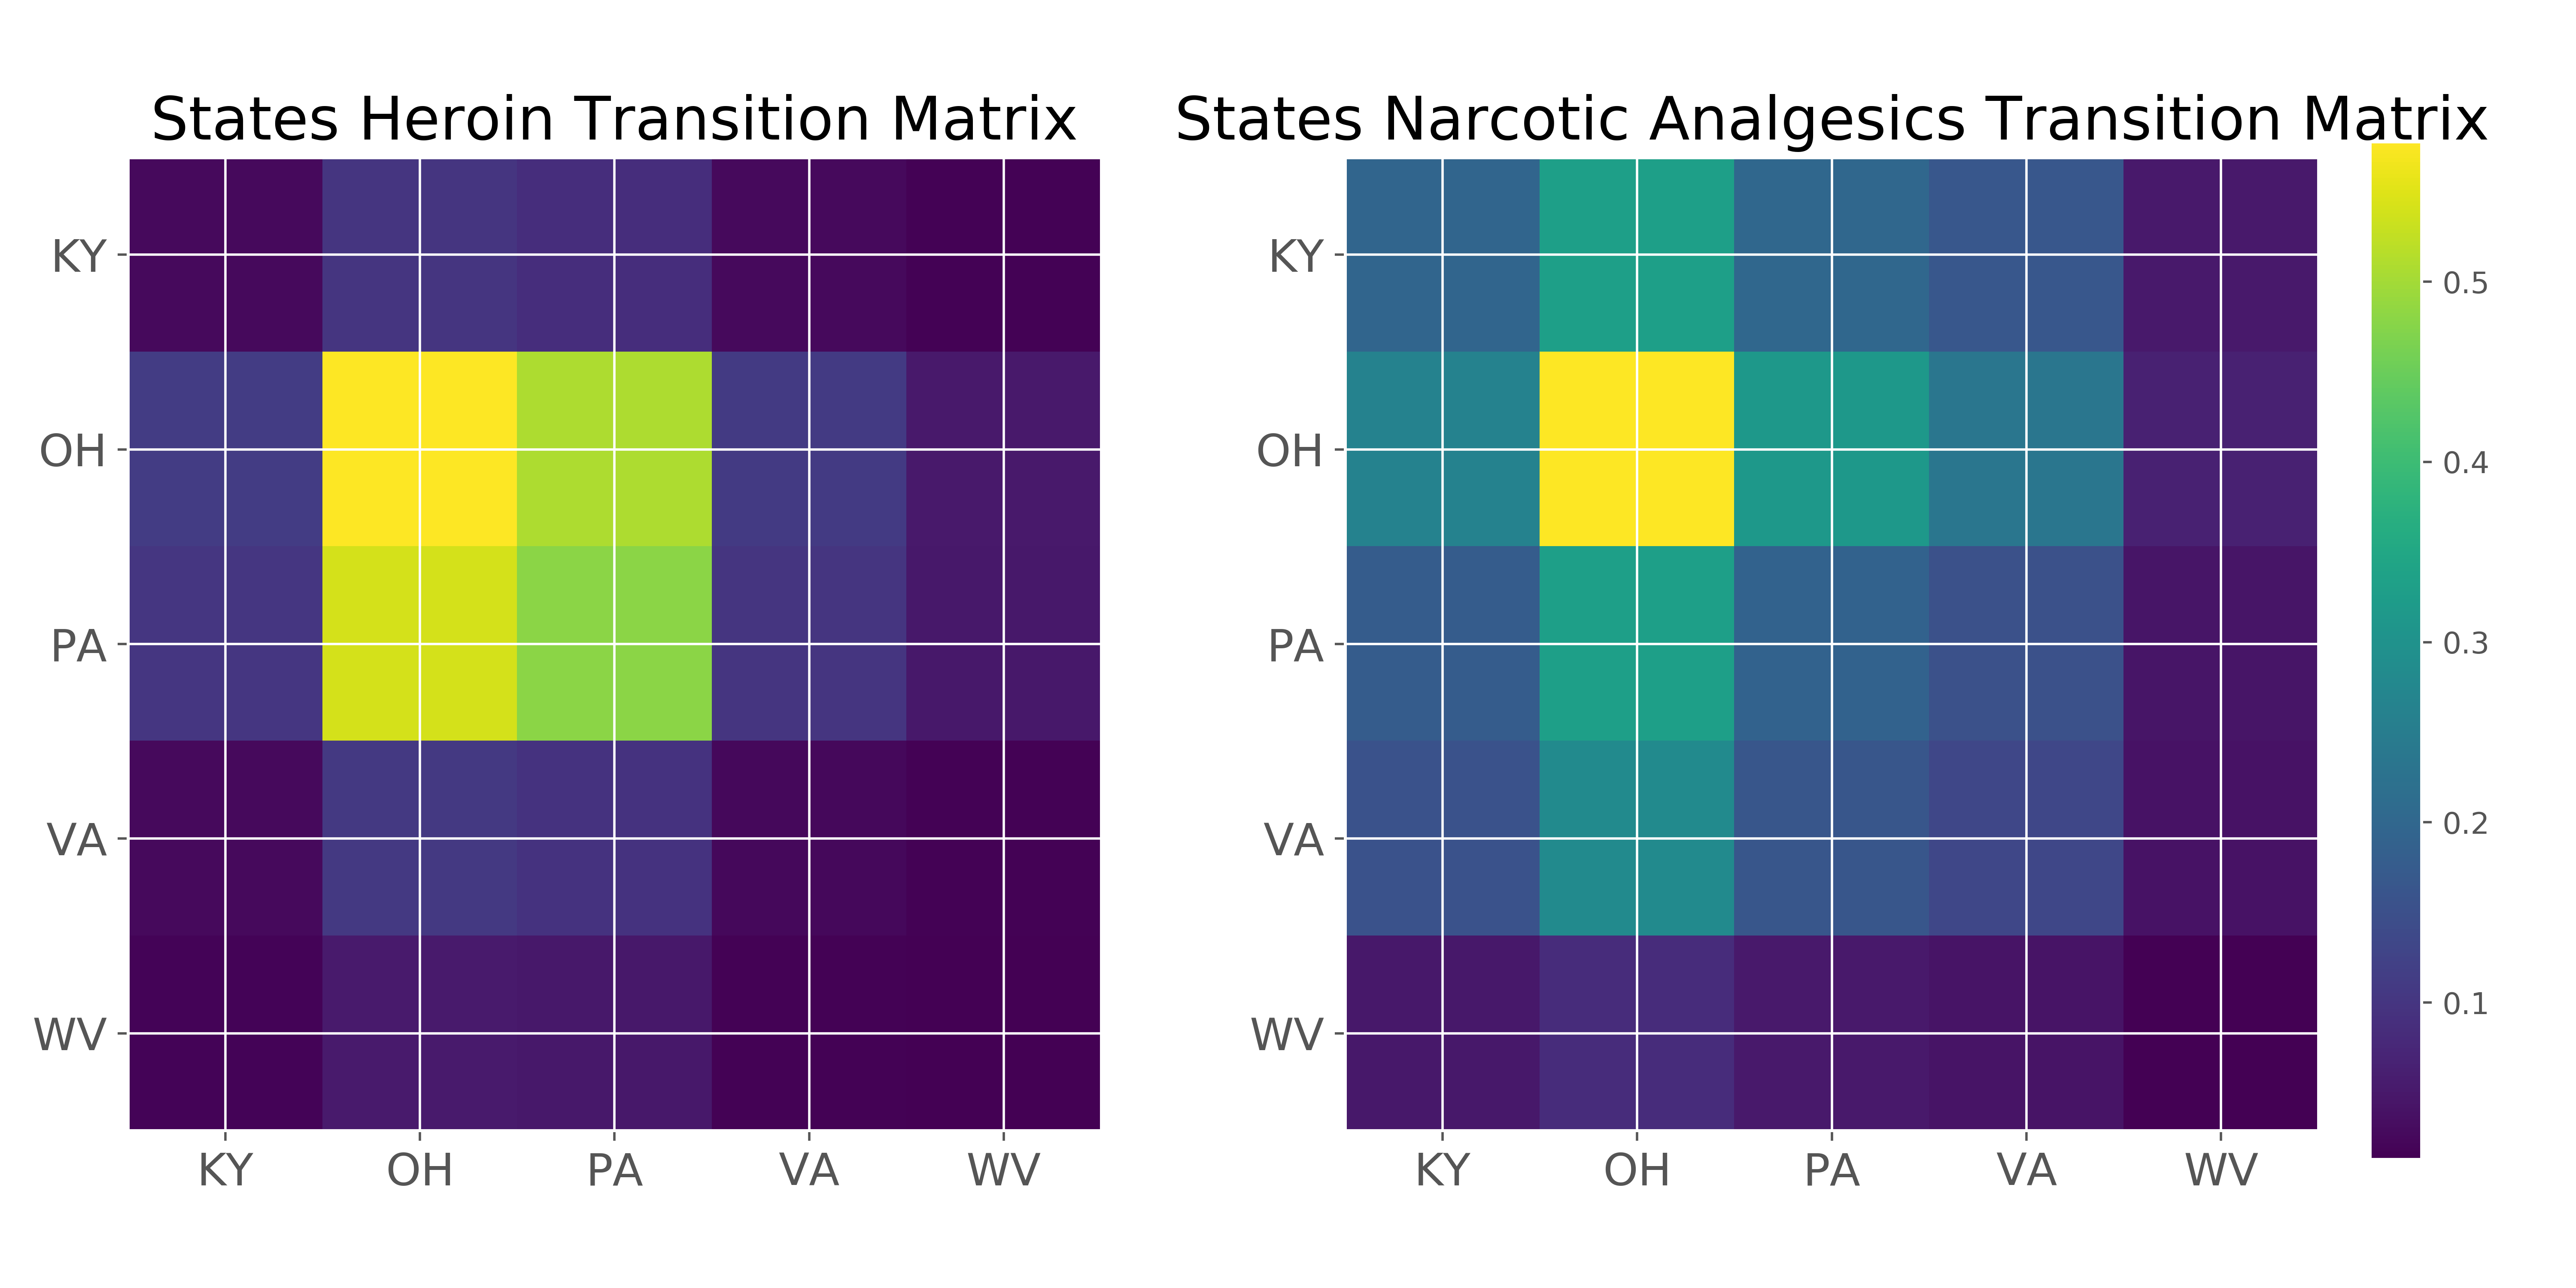
\includegraphics[width=\textwidth]{4.png}%以pic.jpg的0.5倍大小输出
    \end{minipage}
    }
    \\%换行控制

    \caption{name of the figure}    %大图名称
    \label{fig:1}    %图片引用标记
\end{figure}

正常的图片:

\begin {figure}[h]
	\centering % 居中显示
	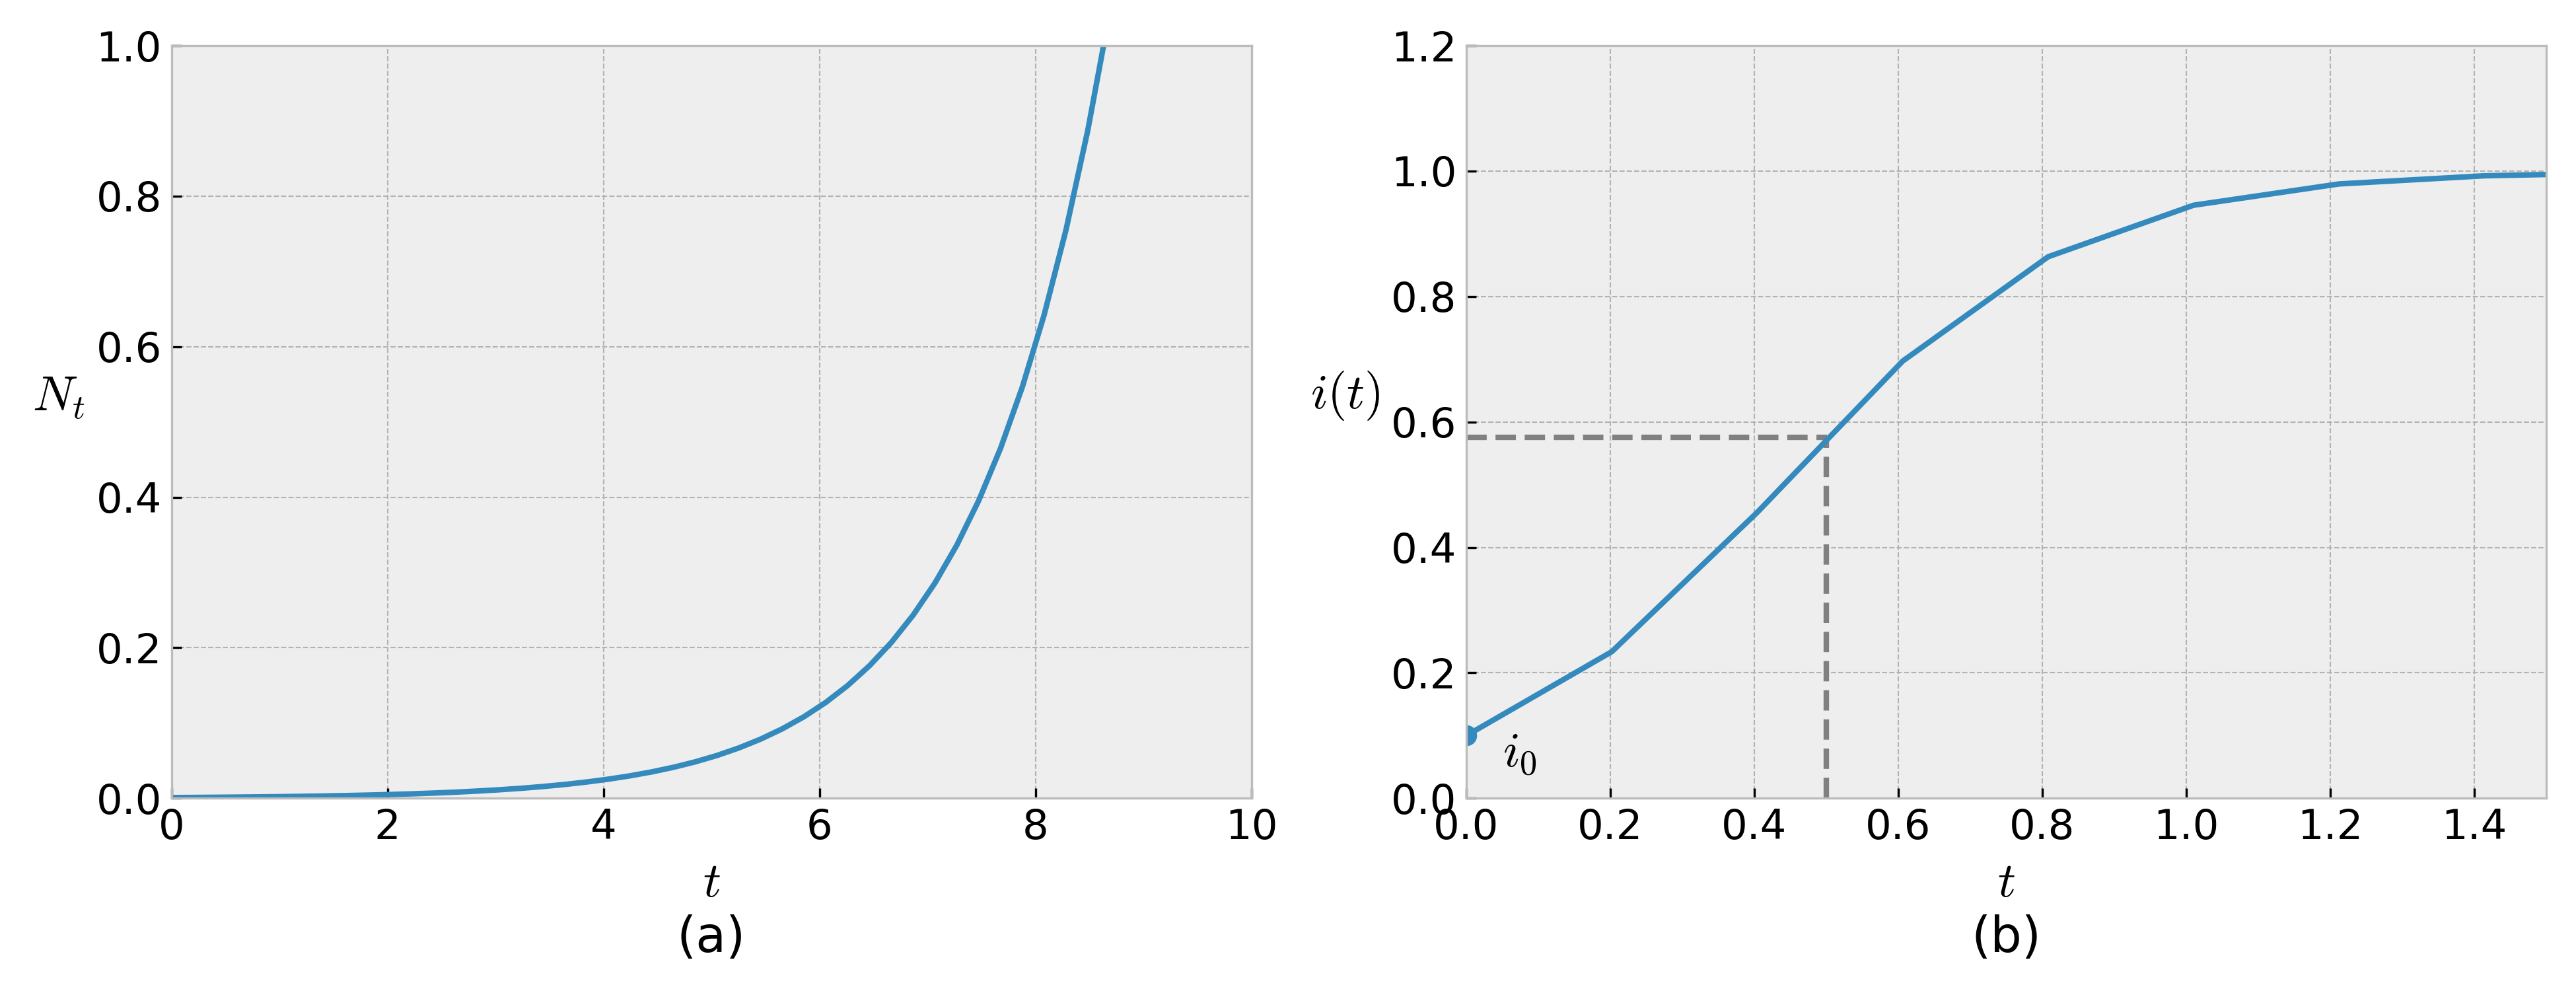
\includegraphics[width=\textwidth]{1.png}
	\caption{Heat map of transition matrix for five states} % 标题
	\label{five}
\end {figure}

\begin {figure}[h]
\centering % 居中显示
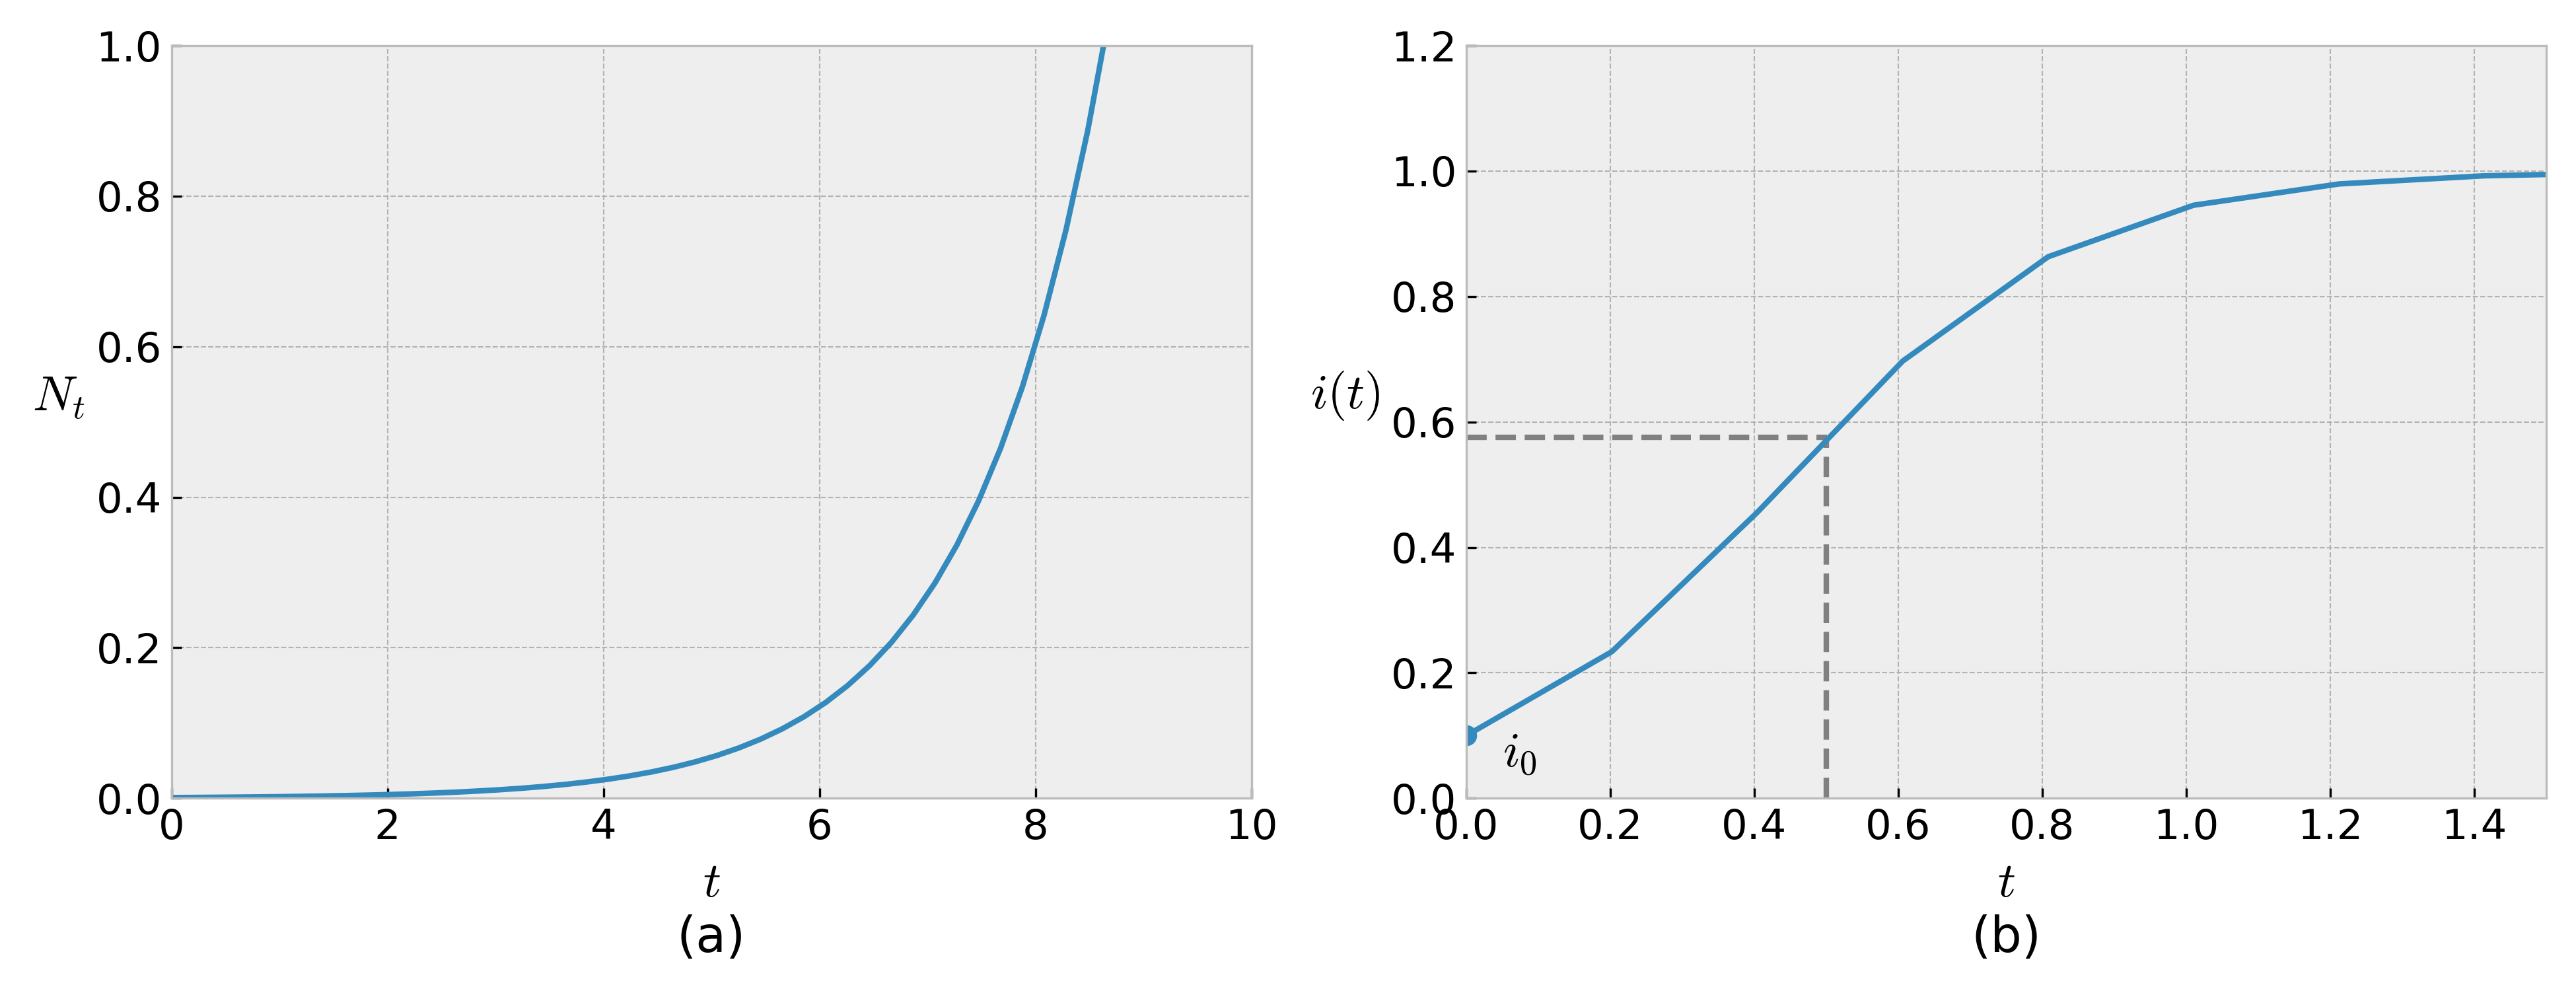
\includegraphics[width=\textwidth]{1.png}
\caption{sdad} % 标题
\label{five}
\end {figure}

\begin{figure}[htbp]
    \centering  %居中
    \subfigure[dsa]{   %第一张子图
    \begin{minipage}{0.4\textwidth}%大小总和超过textwidth则自动换行
    \centering    %子图居中
    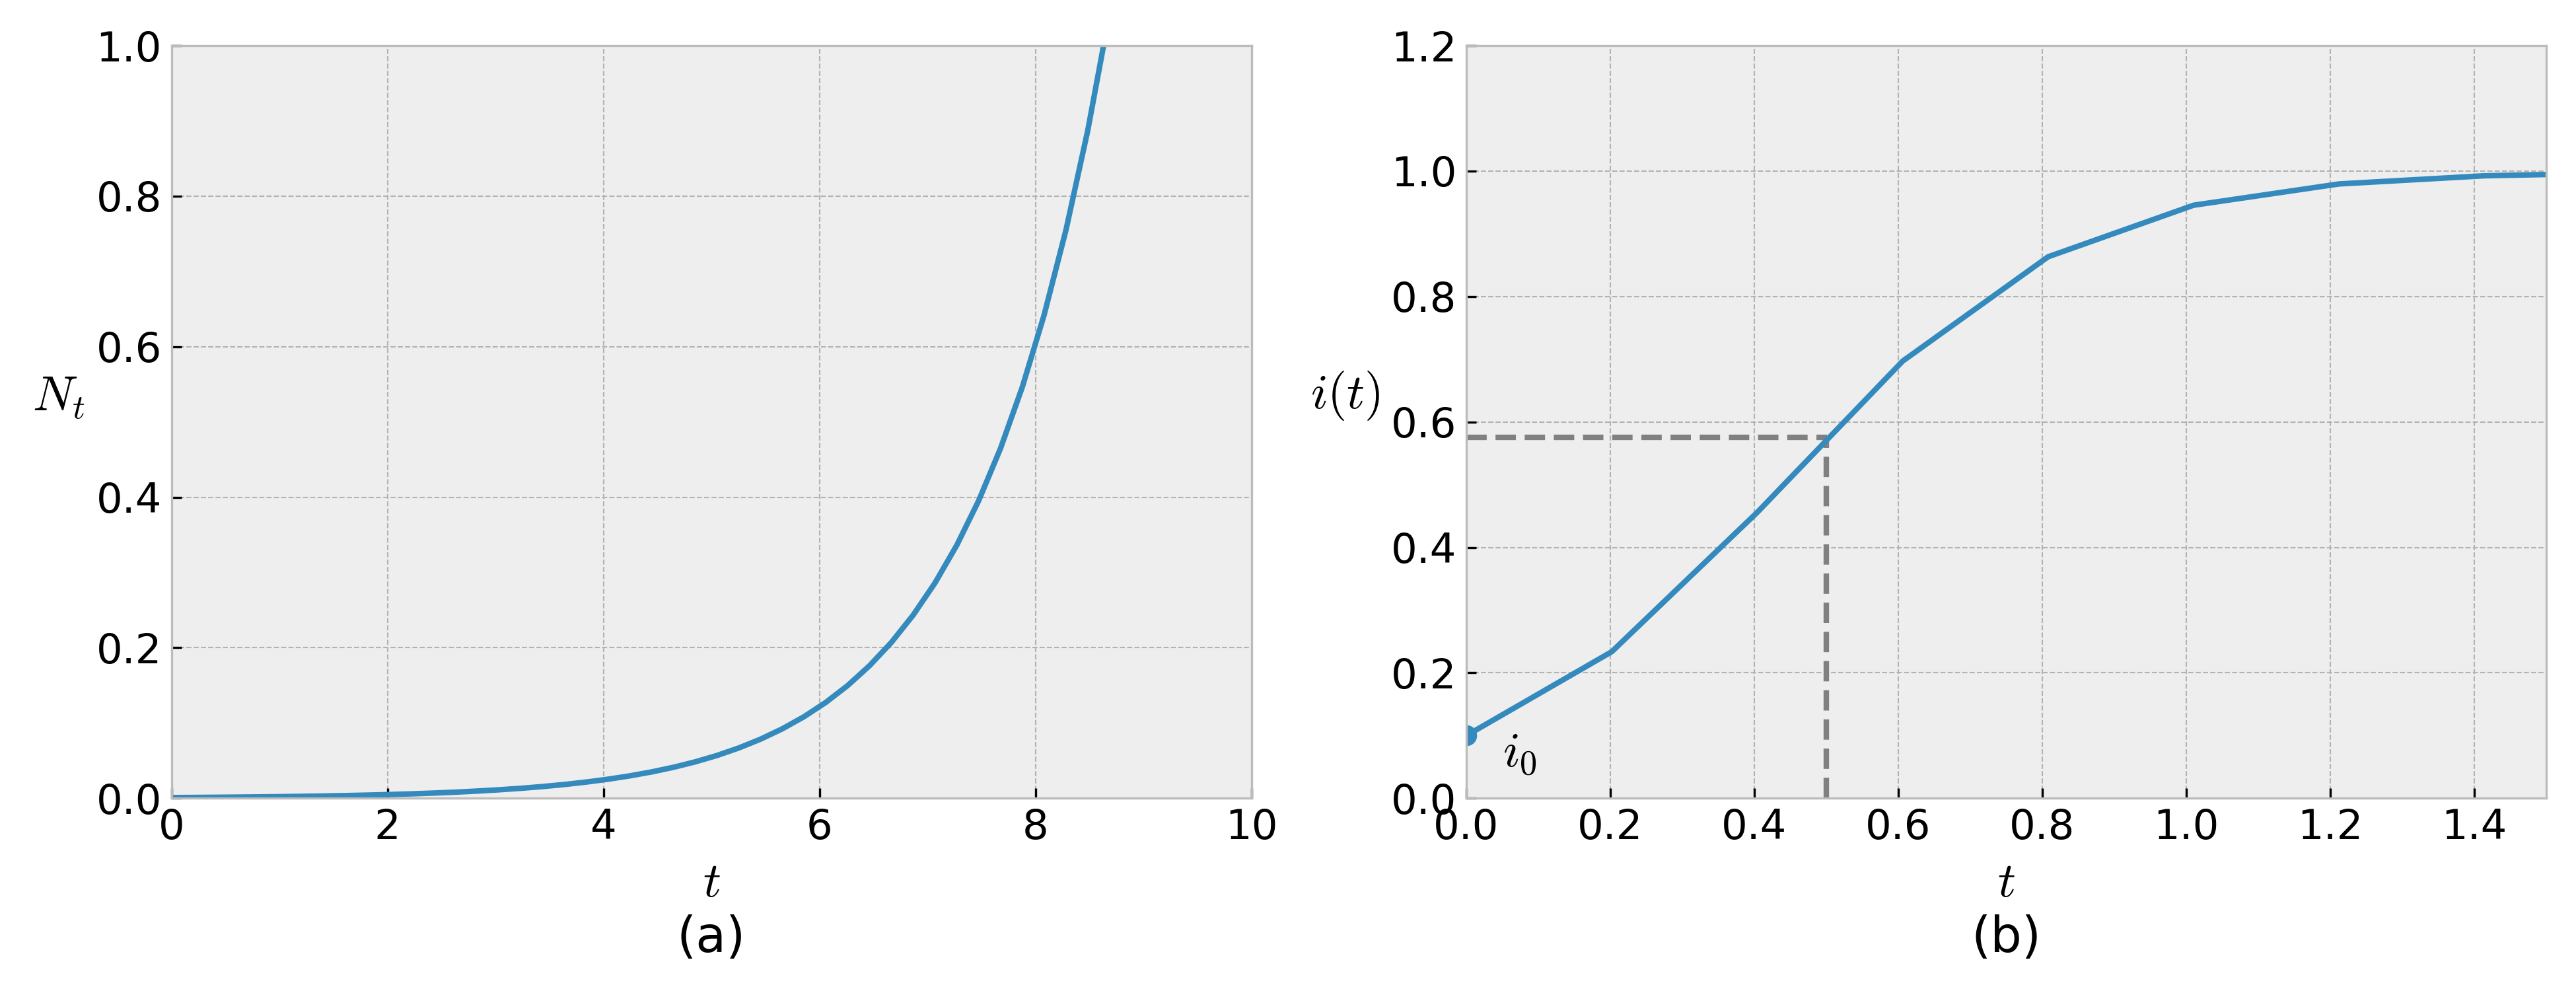
\includegraphics[width=\textwidth]{1.png}  %设置图片的输出大小倍数,这里是0.5倍大小输出
    \end{minipage}
    }
    \subfigure[dsa]{ %第二张子图
    \begin{minipage}{0.4\textwidth}
    \centering    %子图居中
    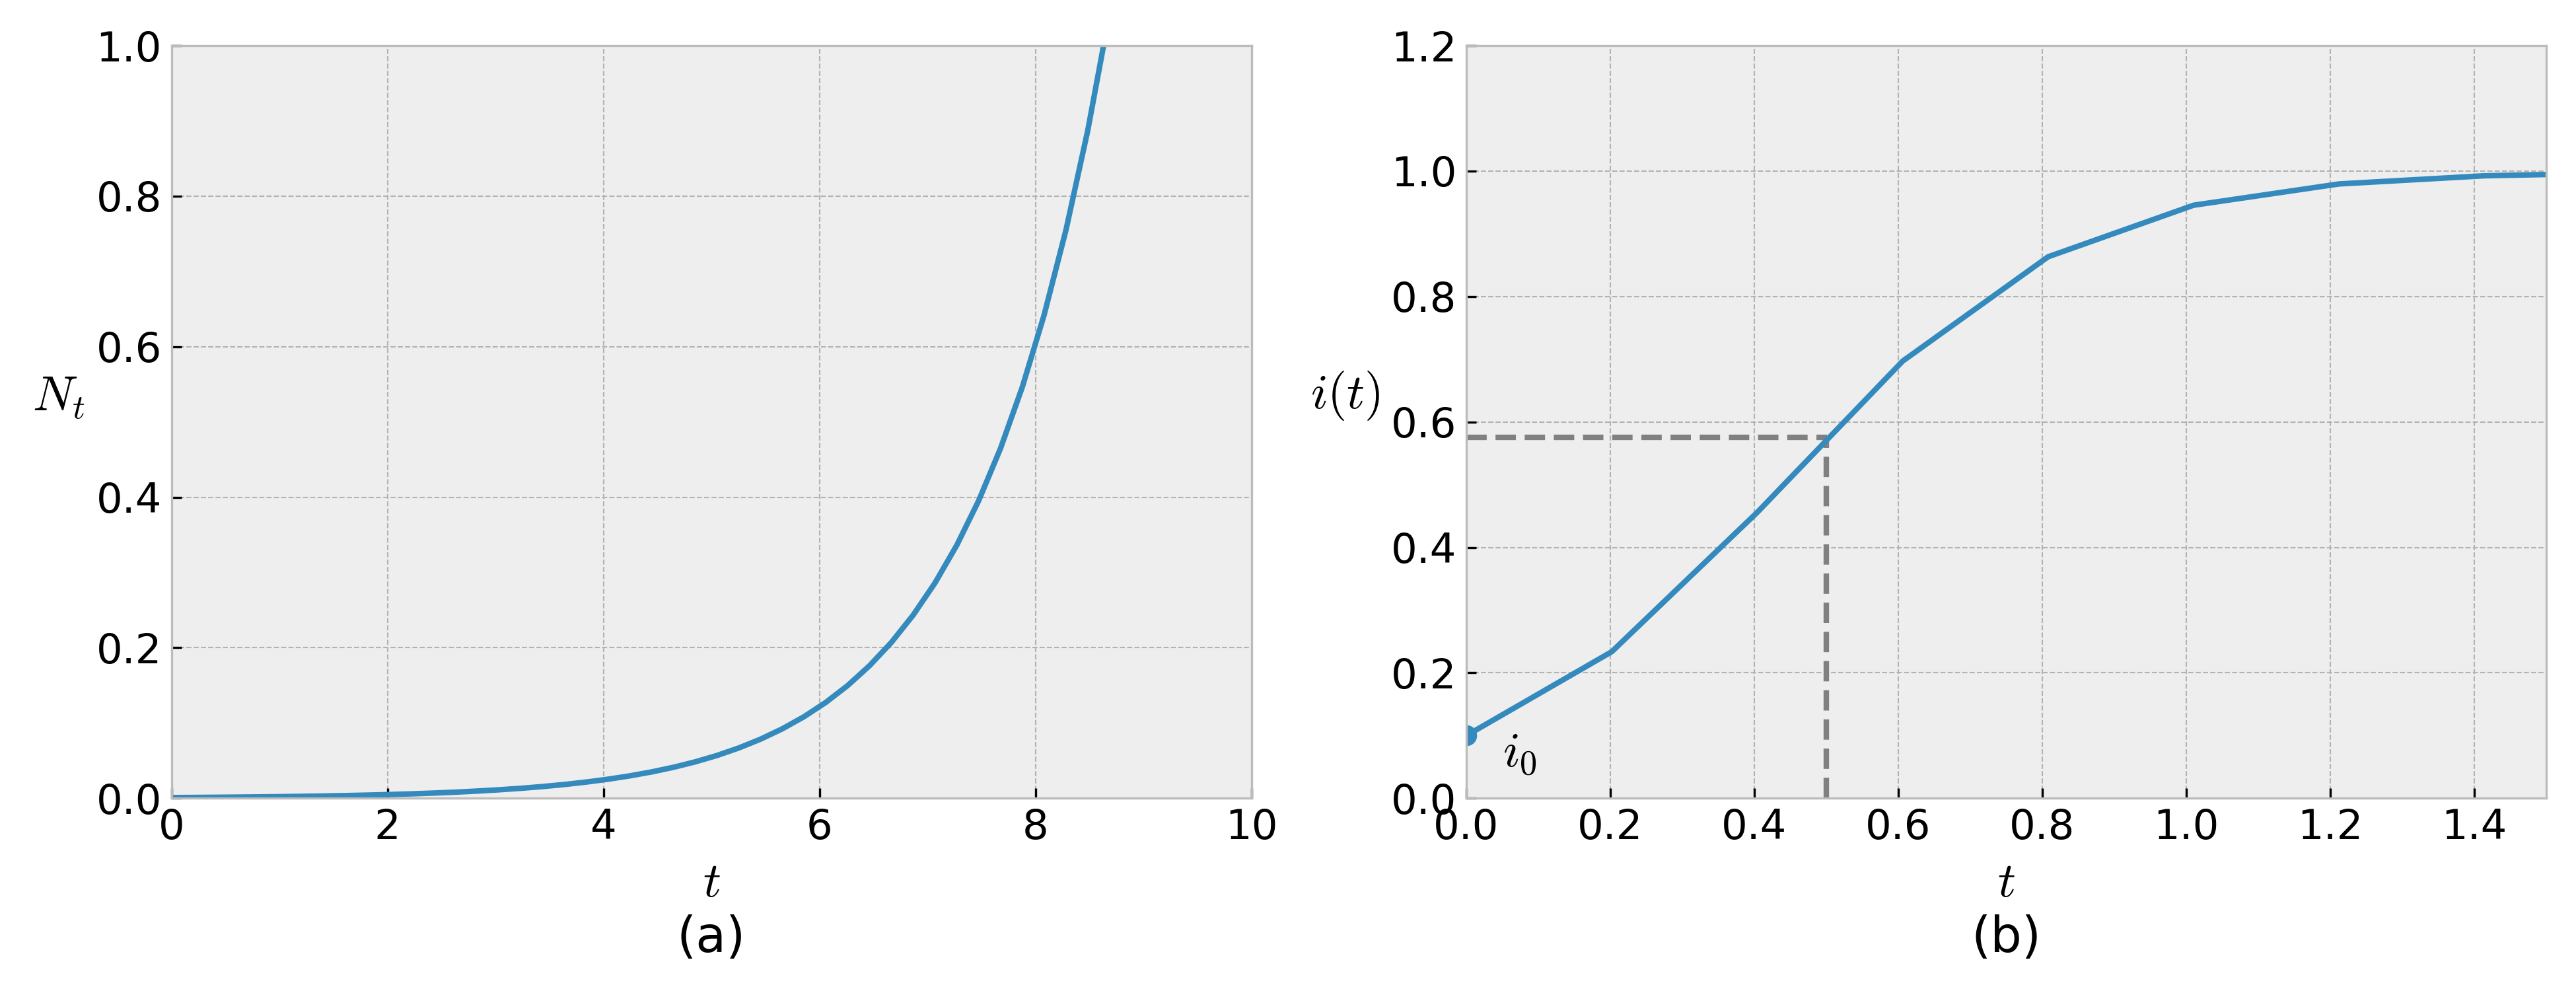
\includegraphics[width=\textwidth]{1.png}%以pic.jpg的0.5倍大小输出
    \end{minipage}
    }\\
    
        \subfigure[zx]{   %子图
        \begin{minipage}{0.8\textwidth}%大小总和超过textwidth则自动换行
        \centering    %子图居中
        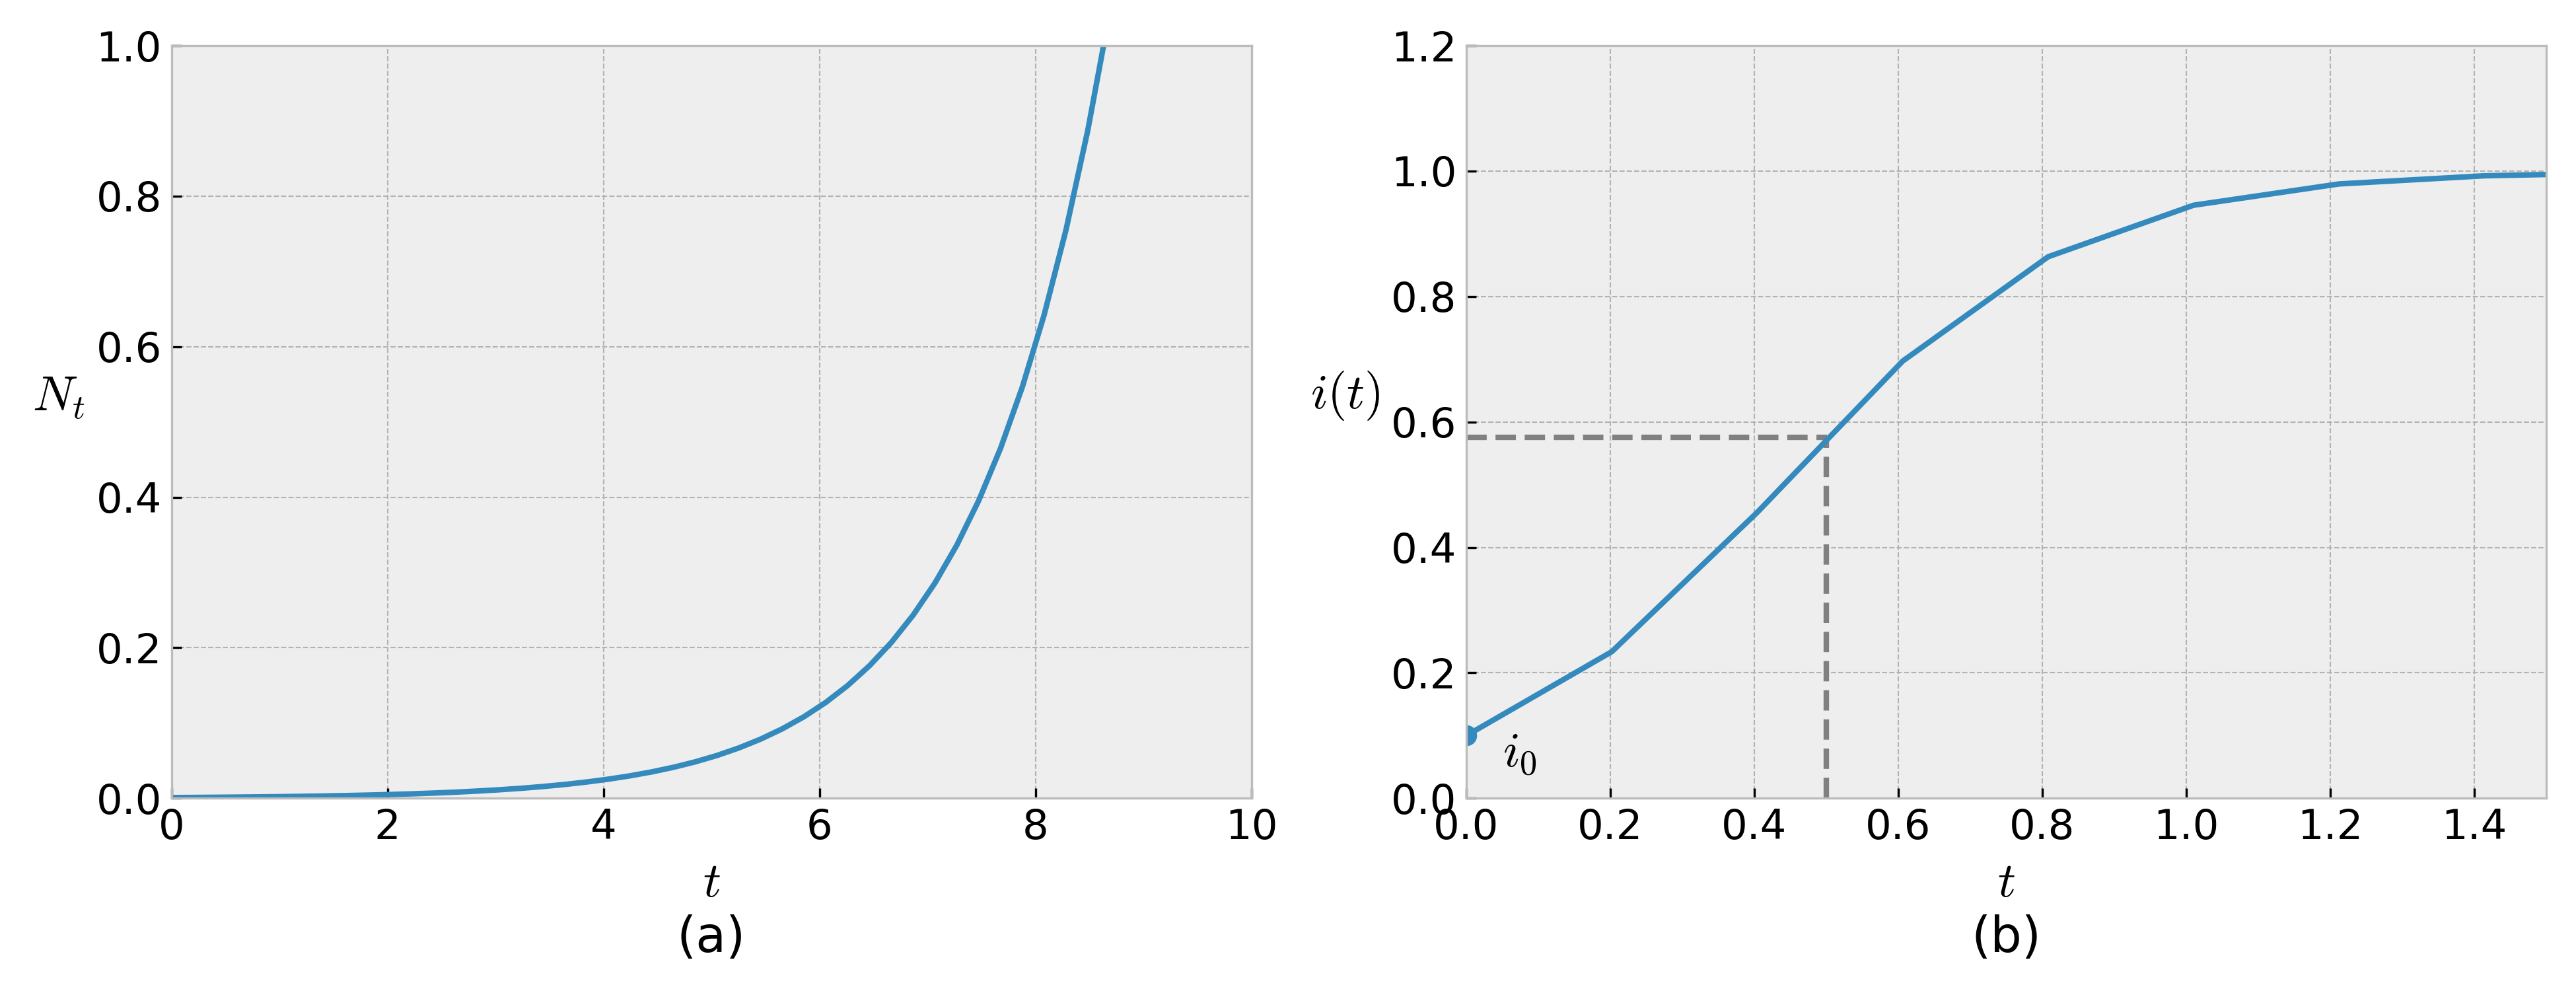
\includegraphics[width=\textwidth]{1.png}  %设置图片的输出大小倍数,这里是0.5倍大小输出
        \end{minipage}
        }
    \caption{name of the figure}    %大图名称
    \label{fig:1}    %图片引用标记
\end{figure}
\end{document}